\documentclass[11pt]{article}
\usepackage{times}
\usepackage[dvips]{graphicx}
\usepackage{float}
\usepackage{latexsym,fullpage,amsmath, listings}
%\usepackage{latexsym,fullpage,times}
\usepackage{float,array}
\usepackage[colorlinks]{hyperref}

\newcommand{\onefig}[4]{
\begin{figure}[htb]\hrule
\vspace{3pt}
\begin{center}
\includegraphics[scale=#4]{#1}
\caption{#2} \label{#3}
\end{center}
\vspace{3pt} \hrule
\end{figure}
}

\begin{document}

\begin{center}
{\Large ME/IE/CS 558 -- Spring 2018}\\ \vspace{12pt} {\large
Assignment 3:  Part 2}\\ \vspace{12pt} {\em Due at midnight on March 23rd, 2018}
\end{center}

{\bf For all assignments:} {\em Unless specifically indicated, you
are free to use any publicly available sources: papers, books,
programs, online material, etc. -- as long as you clearly indicate
and attribute the origin of the information.}

\subsection*{The Task}

In this multi-part assignment, you have to design a program that reads in
$(x,y)$ coordinates of random points and constructs their (otherwise 
unconstrained) Delaunay triangulation and a Voronoi diagram.  
In Part 1 of the assignment, you  designed a data structure for the triangulation, 
and constructed an uncosntrained triangulation (not Delaunay) for a given set of points in a plane.  
In Part 2 of the assignment, you will transform the triangulation into the Delaunay triangulation using edge-flipping algorithm.


\subsection*{The Challenge}



Recall that the essence of the edge flipping step is to
identify a `reversable' edge in a convex quadrilateral and flip it
to a Delaunay edge for this quadrilateral (see Figure \ref{fig:quad}).
Design a data structure that will allow efficiently keeping track
of which edges have been flipped and which have not been flipped.
Recall that every time an edge is flipped, some new edges may
become reversable and must be reexamined.  The `edge-flipping'
algorithm continues flipping edges in the triangulation until no
more reversable edges remain. Your algorithm should not take more
than $O(n^2)$ running time.

\begin{figure}[tbh]
\centering
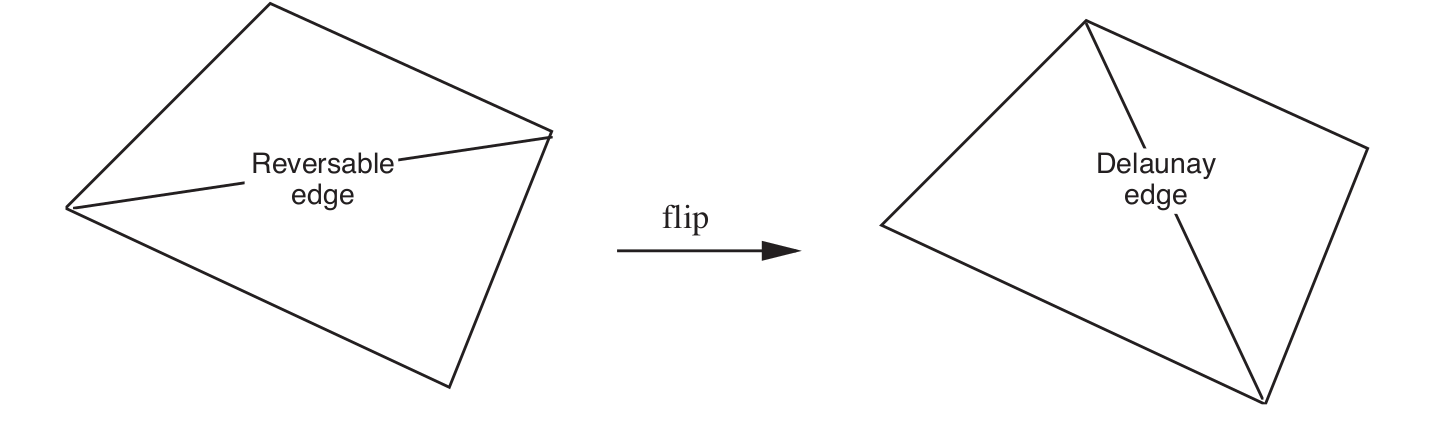
\includegraphics[scale=0.3]{quad.png}
\caption{The flipping procedure for a convex quadrilateral}
\label{fig:quad}
\end{figure}

%\onefig{quad.png}{The flipping procedure for a convex
%quadrilateral}{quad}{1}

\newpage
\subsection*{Deliverables}

\begin{description}
\item [Analysis -- 50 points]\hfil\\ 
Provide all  details of your data structures and algorithms
necessary for an implementation. 
%Design the crucial tests used in
%constructing a valid triangulation and performing edge flipping.
Estimate the running time of your algorithms, making sure that the
total running time does not exceed $O(n^2)$.


\item[Program -- 50 points] \hfil\\ Implement your data structures
and the algorithm.    Assume that  the input file  
{\em testPoints.txt}  contains the list  of test points, each point described by its $x$ and $y$ coordinates:
 $x\;y$

% Your program should plot the triangulation (either the edges or the triangles or both) on the screen. 
Your program will be called from command line as

\begin{lstlisting}

>> python delaunay.py filename

\end{lstlisting}

Coordinates file stores n 2D points with the below format.

\begin{lstlisting}

x1 y1
x2 y2
...
xn yn

\end{lstlisting}

Your program should print out the number of triangles, edges, and vertices in the triangulation 
and plot the triangulation (either the edges or the triangles or both) on the screen.
For example, for the following points.txt file

\begin{lstlisting}
2.538509	8.226810
8.460951	7.686782
4.859579	9.416016
6.957145	2.587729
6.151283	5.697434
5.870937	8.468682
8.384895	0.096601
2.727876	3.340728
1.996933	2.157899
0.741161	2.732918
\end{lstlisting}

Your program should print the below information.
\begin{lstlisting}
number of triangles = 12
number of edges = 21
number of vertices = 10
\end{lstlisting}

Your program should also plot the delaunay triangulation (see Figure \ref{fig:delaunay}).

\begin{figure}[H]
  \centering
  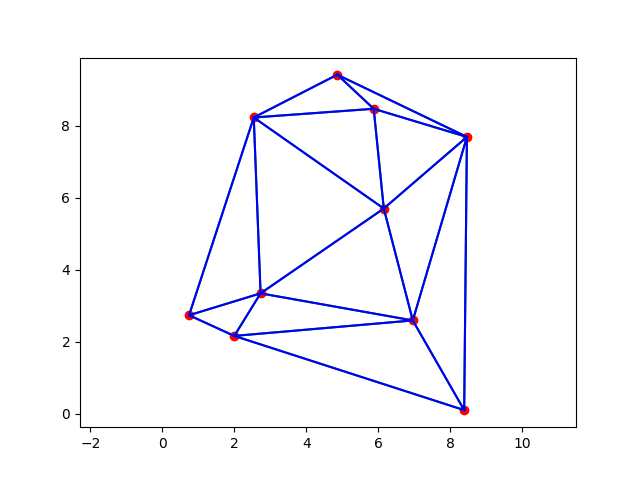
\includegraphics[scale=0.5]{points2.png}
  \caption{Delaunay triangulation}
  \label{fig:delaunay}
\end{figure}

Test your program on a variety of inputs, including the test files posted on the course webpage.
Explain how you chose your tests. 


As usual, the overall structure of your program should be explained and documented; your code should contain appropriate comments.
\end{description}
 
 

\subsection*{Deliverables}

Please use the course website to submit a single  zip  named   FirstName\_LastName\_HW32.zip
The zip archive should contain:  (1) the analysis portion of the assignment,  (2)  the documented python source file, and (3) a PDF readme file  specfying the instructions for running the code.  It should also include at least 1 sample run with input and output,  and specify any specific dependencies or requirements of your code.  

\end{document}


